%%%%%%%%%%%%%%%%%%%%%%%%%%
%%  Capítulo 2: Fundamentos de estructuras de banda prohibida electromagnética (EBG)}  %%
%%%%%%%%%%%%%%%%%%%%%%%%%%

%%%%
\section{Introducción: Metamateriales, materiales periódicos y EBGs}
\label{sec_resenia_metamateriales}
%%%%

% Caloz, ^pag 17
% Caloz Pag 20
% Caloz pag 83, diferencia con filtros
% Pozar, pag 380
% Pozar, p 424. Stepped impedance filters.
% Pozar, bandstop filter design, pag 440
% TABLA interesante: Baccarello, Paulotto, impreso.
% stack de capas o cristal? Brown, McMahon, Parker. Ademas linda foto.
% Relación con soft-hard surfaces. Gao, chen, wang, yang-
% Discusión terminológica: Oliner.
% ITOH, Pediodic structures.
% DGS, tesis de ABIDIN, pag2. Tiene intro histórica.
% ABIDIN, tesis, pagina 16: Def de EBG. imagen interesante.
% Venkateswaran, algunos ejemplos de EBGs.
% Importancia de EBGs. Venkateswaran tesis, pag 1.
% Algo de intro: Pagina 4, tesis Zheng.

La definición de metamaterial aún está en discusión aunque, en términos generales, la más aceptada indica que son estructuras electromagnéticas artificiales efectivamente homogéneas que presentan propiedades que no se encuentran en la naturaleza \cite{Caloz:ElectromagneticMetamaterials}. Los materiales EBG (de banda prohibida electromagnética, \textit{Electromagnetic Bandgap}), PBG (de banda prohibida fotónica, \textit{Photonic Bandgap}) o cristales fotónicos son un tipo de estructura artificial, dieléctrica o metalodieléctrica, en algunos casos clasificadas como metamateriales, con capacidades para controlar ondas electromagnéticas \cite{Engheta:Metamaterials} a partir de una variación periódica en el espacio de la constante dieléctrica $\epsilon$. Tienen la capacidad de permitir la propagación en direcciones determinadas, o de impedirla completamente, debido que presentan una banda prohibida electromagnética, concepto análogo al de banda prohibida electrónica, que controla el movimiento de ondas de electrones que viajan en un potencial periódico cristalino.

La condición de homogeneidad efectiva de los metamateriales se cumple si las estructuras que forman al EBG están a distancias mucho menores a la longitud de onda guiada incidente, $\lambda_g$ \cite{Caloz:ElectromagneticMetamaterials}, de forma que la naturaleza de la estructura básica que se periodiza, denominada celda unitaria, determine parámetros constitutivos ($\epsilon$ y $\mu$) electromagnéticamente uniformes en la dirección de propagación, para la frecuencia de interés. En función de la relación entre estos parámetros constitutivos, las ondas electromagnéticas que lo atraviesan tienen comportamientos diferentes, como se muestra en la figura \ref{fig:tablamuepsilon}. El estudio de estructuras periódicas permitió, entonces, la fabricación de materiales con características en los cuatro cuadrantes del plano $\mu$-$\epsilon$.

\begin{figure}[htp]
	\centering
	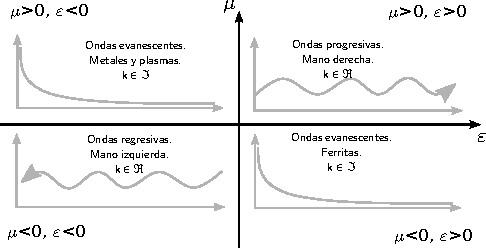
\includegraphics[width=0.6\textwidth]{Fundamentos/OndasSegunEyU.pdf}
	\caption{Tipos de ondas en función de los valores de $\epsilon$ y $\mu$.}
	\label{fig:tablamuepsilon}
\end{figure}


A fines del siglo XVIII, el físico estadounidense David Rittenhouse observó que algunos de los colores del espectro de luz visible desaparecían cuando una lámpara era vista a través de un pañuelo \cite{Rittenhouse:OpticalProblem}, mostrando por primera vez que un medio discontínuo puede presentar propiedades de transmisión diferentes en función de la frecuencia incidente. El estudio teórico del comportamiento de ondas electromagnéticas en medios periódicos comenzó a principios del siglo XX, aunque no fue hasta finalizada la segunda guerra mundial que se formalizaron algunos conceptos. Ya en 1919, Guglielmo Marconi y Charles Samuel Frankin utilizaron una estructura de conductores horizontales que operaban como una superficie reflectiva para cierta frecuencia, que podría considerarse la primera superficie selectora de frecuencias (FSS).
% Historia: FSS > EBG, e Taylor & Francis, Pag 30-4.

En 1946, Louis Brillouin publicó su libro sobre ondas mecánicas, "\textit{Wave propagation in periodic structures: Electric filters and crystal lattices}" \cite{Brillouin:WavePropagation}, donde demostró que un arreglo periódico impone restricciones a los vectores de onda $\vec{\gamma}$ que pueden propagarse en él, dado que el mismo establece condiciones de contorno para los modos permitidos. Aquellas ondas que no cumplen las condiciones derivadas de la periodicidad de la estructura, no son capaces de propagarse.

En 1968, el físico ruso Viktor Veselago describió por primera vez, de forma teórica, la posibilidad de que existieran sustancias naturales con índice de refracción negativo, denominados LHS (\textit{Left Handed Substances}, sustancias de mano izquierda), cuya permitividad eléctrica y permeabilidad magnética fueran simultáneamente negativas, de modo que la velocidad de fase de una onda que se propagara por ese medio resultara antiparalela a la velocidad de grupo. Treinta años más tarde, a fines de la década de 1990, Smith propuso propuso la primera forma de fabricación de un medio con esas características en una banda limitada de frecuencia, utilizando SSRs (\textit{Split-ring resonators}, resonadores de aro dividido), responsables de la permeabilidad magnética negativa, y cables conductores, responsables de la permitividad eléctrica negativa, ubicados en forma periódica, y estudiados previamente por Pendry (Figura \ref{fig:Pendry}). Recién en el año 2000 se construyó el primer metamaterial sobre las propuestas de Smith, mostrado en la figura \ref{fig:metamaterial-de-smith}, y varios experimentos confirmaron refracción negativa en los mismos. Hasta la fecha, no han sido encontrados materiales naturales con este comportamiento.

\begin{figure}[htp]
	\centering
	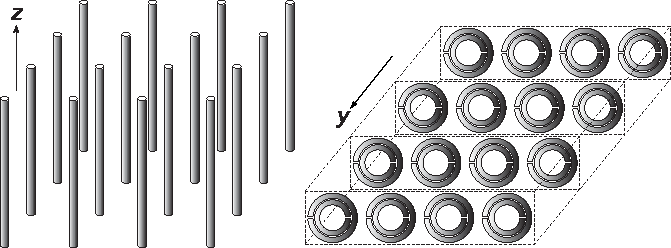
\includegraphics[width=0.8\textwidth]{Fundamentos/pendry.pdf}
	\caption{Metamateriales propuestos por Pendry. A la izquierda, un WSM (\textit{Wire Screen Medium}), que posee $\epsilon<0$ y $\mu>0$ cuando el campo eléctrico es longitudinal a los cables, para un rango de frecuencias determinado. A la derecha, un medio de SRR, que posee $\epsilon>0$ y $\mu<0$ cuando el campo magnético es perpendicular al eje de los anillos, para una frecuencia determinada \cite{Caloz:ElectromagneticMetamaterials}.}
	\label{fig:Pendry}
\end{figure}

\begin{figure}[htp]
	\centering
	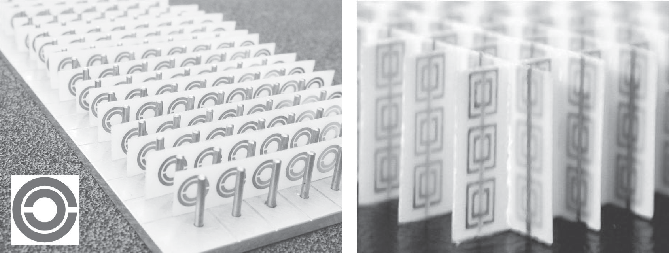
\includegraphics[width=0.8\textwidth]{Fundamentos/metamateriales-smith.pdf}
	\caption{Estructuras metamateriales propuestas por Smith \cite{Caloz:ElectromagneticMetamaterials}.}
	\label{fig:metamaterial-de-smith}
\end{figure}

En el contexto de una línea de investigación, en principio, independiente de los trabajos previos de Veselago, la primera descripción de estructuras dieléctricas periódicas con una banda prohibida completa fue dada, en 1990, por Ho, Chan y Soukoulis, en Iowa, Estados Unidos, quienes propusieron un arreglo periódico de esferas dieléctricas, dispuestas en forma de capas. Para un rango amplio de radios de esferas, el efecto de banda prohibida se daba en todas direcciones. Posteriormente, Yablonovitch divisó una estructura cristalina simétrica de más fácil fabricación, que consistía en la producción de tres agujeros cilíndricos en un prisma dieléctrico, repetido periódicamente. Demostró, además, usando dichas estructuras, que la existencia de una banda prohibida electromagnética podía ser predicha teóricamente, en base, principalmente, a la constante de periodicidad del dieléctrico artificial.

Los trabajos de Yablonovitch, en estructuras de banda prohibida electromagnética, y Pendry, en metamateriales de índice de refracción negativo, se hicieron sobre estructuras con banda de interés en microondas, pero bajo modelos fotónicos, gracias a la linealidad de las ecuaciones de Maxwell. Esto permitió el uso de distintas técnicas conocidas y desarrolladas durante el siglo XX en microondas para el diseño de materiales fotónicos de estas características a partir de finales de la década de 1990, principalmente en ámbitos de investigación de ciencias básicas.

Al mismo tiempo, comenzaron los estudios sobre las denominadas "superficies electromagnéticas" (\textit{electromagnetic surfaces}), que consisten en superficies texturadas, generalmente conductoras (en contraposición a los trabajos tridimensionales) que imponen condiciones de contorno particulares, capaces de lograr cambiar la polarización de una onda incidente, influir sobre las ondas de superficie y controlar la fase de reflexión, actuando como estructuras de banda electromagnética bidimensionales. La más simple consiste en una placa metálica coarrugada, como la mostrada en la figura \ref{fig:superficie-coarrugada}, de forma que las variaciones de altura sean de $\lambda/4$, que puede comportarse como una "superficie blanda" (\textit{soft surface}) o una "superficie dura" (\textit{hard surface}), en función de la polarización de la onda que se propaga \footnote{Si el campo eléctrico es perpendicular a las ranuras, la hendidura de profundidad $\lambda/4$ actúa como una línea de transmisión de cuarto de onda cortocircuitada, lo que, en la parte superior de las ranuras, se convierte en un circuito abierto, actuando como una superficie de alta impedancia. Si, en cambio, el campo eléctrico es paralelo a las ranuras, la impedancia que presenta es baja.}. Los primeros trabajos sobre estructuras bidimensionales con comportamiento de banda prohibida electromagnética dieron lugar a las denominadas FSS (\textit{Frequency Selective Surfaces}, superficies selectoras de frecuencias) \cite{Munk}. En 1999, Sievenpiper \cite{Sievenpiper:Thesis} propuso, en su tesis doctoral, estructuras superficiales compactas de alta impedancia, de manera que no fuera necesario el uso de una distancia de $\lambda/4$ entre la superficie superior y la inferior para lograr el efecto deseado, dado que se cargaba capacitivamente a la estructura \cite{Marcela:Tesis} \cite{Sievenpiper:HIESForbiddenBand}. Estas nuevas superficies periódicas consisten en un arreglo metalodieléctrico de subestructuras denominadas "hongos" (\textit{mushrooms}), como se muestra en la figura \ref{fig:sievenpiper}, y proveen condiciones de borde de alta impedancia para polarizaciones TE y TM al mismo tiempo.

\begin{figure}[H]
	\centering 
	\subfigure[Superficie coarrugada tradicional]{
		\label{fig:superficie-coarrugada}
		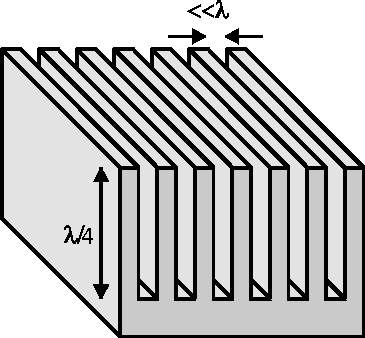
\includegraphics[width=0.35\textwidth]{Fundamentos/superficie-coarrugada.pdf}}
	\hspace{30pt}
	\subfigure[Superficie propuesta por Sievenpiper \cite{Sievenpiper:Thesis}]{
		\label{fig:sievenpiper}
		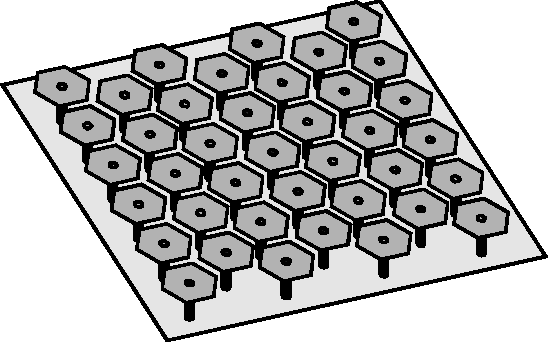
\includegraphics[width=0.45\textwidth]{Fundamentos/sievenpiper.pdf}}
	\caption{Superficie coarrugada tradicional para lograr superficies blandas y duras, y superficie propuesta por Sievenpiper \cite{Sievenpiper:Thesis}.}
	\label{fig:sievenpiper-comparacion}
\end{figure}

El principal interés práctico de las estructuras propuestas por Sievenpiper radica en que actúan como conductores magnéticos artificiales, es decir, tienen una fase de reflexión nula para ondas incidentes, al mismo tiempo que presentan una banda prohibida electromagnética para las ondas de superficie. Esto se puede explicar a baja frecuencia considerando un modelo cuasiestático, dado que la distancia entre los parches conductores de la capa superior dan lugar, debido a la distancia que los separa, a una capacidad. La corriente que circula entre parches vecinos por efecto de una onda de superficie da lugar, análogamente, a una inductancia. Cuando el circuito resonante paralelo que forman resuena, la impedancia aumenta, dando lugar a una banda prohibida. Para frecuencias menores a la de resonancia, la superficie es inductiva y soporta ondas TM, mientras que para frecuencias mayores a la misma, la superficie es capacitiva, lo que permite la existencia de ondas TE. La explicación para las bandas prohibidas en mayores frecuencias requiere un análisis de redes y campos.

En base a la propuesta de Sievenpiper, y en búsqueda de una mayor facilidad de fabricación, en 2001 Yang propuso la aplicación de los conceptos de superficies selectoras de frecuencias (FSS) con la intención de lograr un comportamiento similar, pero evitando el uso de vías entre el plano conductor inferior y las estructuras ubicadas en la capa superior. Estas nuevas estructuras uniplanares son de más fácil fabricación, reduciendo al mismo tiempo el costo, aunque los anchos de banda prohibida electromagnética para ondas de superficie se redujeron ampliamente. El bajo costo, el bajo peso y el bajo perfil de estas estructuras las volvieron de particulares interés en el diseño de antenas.



%\section{Difracción de Bragg}
%\label{sec_bragg}
%%%%%
%% Caloz, pag 19
%% Kamgaing (tesis), pagina22
%\lipsum

\section{Celdas unitarias de cristales bidimensionales}
\label{sec:celdas-unitarias}
En un material periódico se puede definir una red de Bravais, que indica la forma en que los elementos están físicamente dispuestos en la red cristalina. En la figura \ref{fig:direct-lattice}, $\vec{a_1}$ y $\vec{a_2}$ son la base de vectores que permite expresar la posición de cualquier elemento del arreglo como una combinación lineal de coeficientes enteros:

\begin{equation}
R_{n_1,n_2} = n_1 \vec{a_1} + n_2 \vec{a_2}, \quad n_i \in \textbf{Z}, i={1,2}
\end{equation}

La celda unitaria de la red de Bravais se denomina celda de Wigner-Seitz, y restringe la región del espacio más cercana a cada elemento de la red cristalina. Se puede observar, para el caso de una red triangular, en la figura \ref{fig:Wigner-Seitz}.

\begin{figure}[H]
	\centering 
	\subfigure[Red de Bravais correspondiente a una estructura periódica con disposición triangular de los elementos]{
		\label{fig:direct-lattice}
		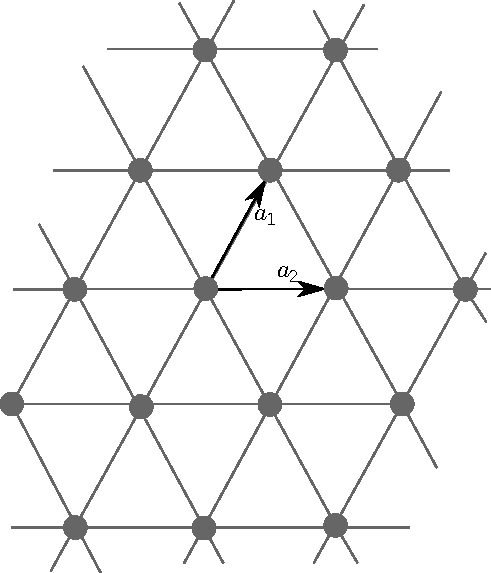
\includegraphics[width=0.45\textwidth]{Fundamentos/direct-and-reciprocal-triangle-lattice.pdf}}
	\hspace{0pt}
	\subfigure[Superposición de la red recíproca y la red directa de Bravais correspondiente a una estructura periódica con disposición triangular de los elementos]{
		\label{fig:reciprocal-lattice}
		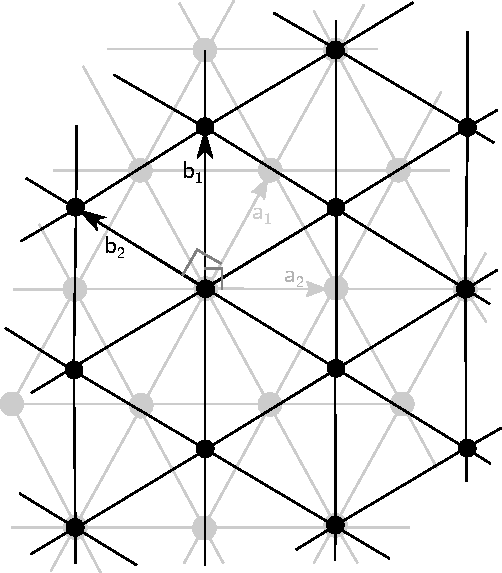
\includegraphics[width=0.45\textwidth]{Fundamentos/direct-and-reciprocal-triangle-lattice-zoom4}}
	\caption{Red de Bravais y red recíproca correspondiente a una estructura periódica. Los vectores $\vec{a_i}$ son los que corresponden a la red directa o red de Bravais, y unen a los elementos físicos del sistema periódico. Los vectores $\vec{b_j}$ son los correspondientes a la red recíproca. Las respectivas redes no están dibujadas a escala y, de hecho, se suelen conceptualizar en espacios diferentes.}
	\label{fig:direct-and-reciprocal-lattice}
\end{figure}

Se puede definir, además, una red dual o recíproca, compuesta de vectores $\vec{b_j}$ tales que cada uno de ellos resulte ortonormal a uno de los vectores $\vec{a_i}$ de la red de Bravais, como se muestra en la figura \ref{fig:reciprocal-lattice}. Esto da lugar a que $a_i$ y $b_j$ sean inversamente proporcionales. El uso de un factor de $2\pi$ permite considerar a la red recíproca como una representación de la red en el espacio de los números de onda $\beta$, de manera que la distancia entre los elementos de la red resulte $2\pi/a$, con $a$ la separación entre los elementos de la red física o de Bravais. Dicho de otra manera, mientras la red de Bravais representa la periodicidad de los elementos que conforman la red física en $(x,y,z)$, la red recíproca es la representación de la misma estructura, pero en el espacio de los vectores de onda, $(\beta_x, \beta_y, \beta_z)$. La red recíproca es también periódica, y sobre ella se pueden buscar, también, celdas unitarias, denominadas regiones de Brillouin o celdas de Wigner-Seitz de la red recíproca, como se muestra en la figura \ref{fig:Celda-unitaria-de-Brillouin}.

Si, además, la celda de Brillouin es lo suficientemente simétrica, se puede definir la denominada zona irreducible de Brillouin, que forma parte de la primer zona de Brillouin, pero está limitada por sus líneas de simetría. Para el análisis de una estructura periódica cualquiera, sólo es necesario analizar esta zona irreducible, dado que el resto son simplemente sus reflexiones espejadas.

\begin{figure}[H]
	\centering 
	\subfigure[Celda unitaria de Wigner-Seitz de la red de Bravais.]{
		\label{fig:Wigner-Seitz}
		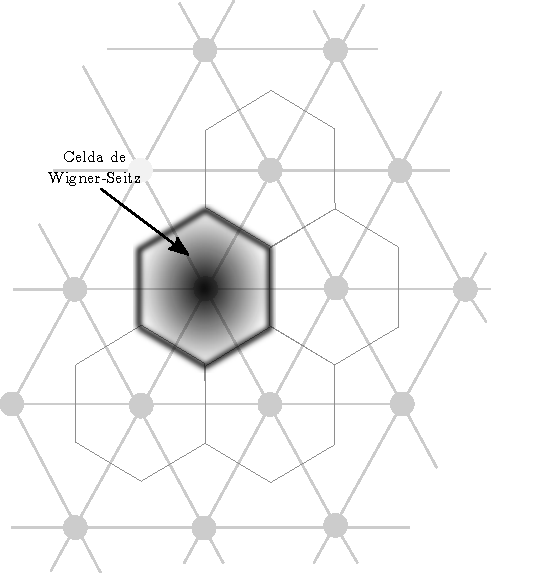
\includegraphics[width=0.45\textwidth]{Fundamentos/direct-and-reciprocal-triangle-lattice-zoom2.pdf}}
	\hspace{0pt}
	\subfigure[Celda unitaria de Brillouin, de la red recíproca, y zona irreducible de Brillouin.]{
		\label{fig:Celda-unitaria-de-Brillouin}
		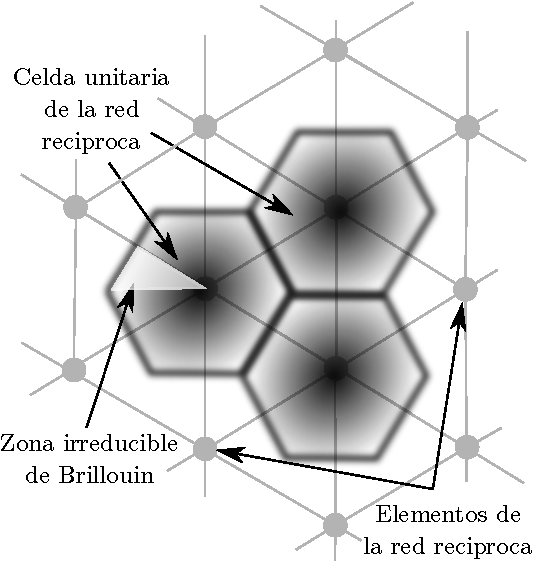
\includegraphics[width=0.45\textwidth]{Fundamentos/direct-and-reciprocal-triangle-lattice-zoom5.pdf}}
	\caption{Celdas unitarias de las redes de Bravais y recíproca.}
	\label{fig:celdas-unitarias}
\end{figure}

Para el caso en que las celdas unitarias son rectangulares, la red recíproca está también dada por una disposición rectangular de elementos, y la zona de Brillouin resulta también cuadrada. La zona irreducible de Brillouin depende de las líneas de simetría, por lo que puede resultar rectangular, a excepción del caso de celdas unitarias cuadradas, donde la mínima unidad que se repite resulta triangular, como se muestra en la figura \ref{fig:rectangulo-cuadrado}.

\begin{figure}[htp]
	\centering
	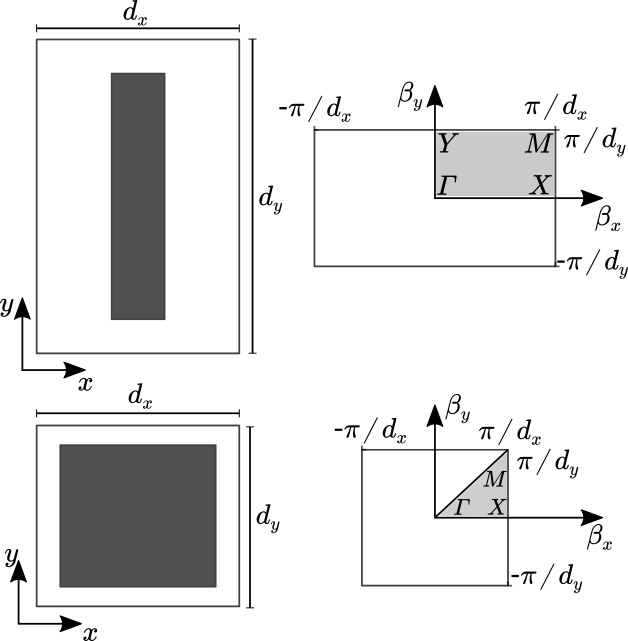
\includegraphics[width=0.5\textwidth]{Fundamentos/rectangulo-cuadradado.pdf}
	\caption{Celda unitaria en el espacio recíproco, y zona irreducible de Brillouin, para celdas unitarias en el espacio de Bravaís rectangulares y cuadradas. Notar que la celda rectangular tiene dos ejes de simetría ortogonales, mientras que la celda cuadrada tiene los mismos ejes, y además con el que corresponde a una recta de $45^{\circ}$.}
	\label{fig:rectangulo-cuadrado}
\end{figure}

\section{Teorema de Bloch-Floquet}
\label{sec:bloch-floquet}

% Floquet es como fourier en el espacio. Taylor and francis, pag 30-5.

El teorema Floquet fue presentado por Gaston Floquet en 1883, y explicita la forma canónica de las soluciones a ecuaciones diferenciales lineales ordinarias de coeficientes periódicos, de la forma $x' = A(t)x$, con $t \in \Re$, $X \in \Re^n$, donde $A(t)$ es una función periódica con periodo $p$. Si $x=\phi(t)$ es solución, entonces también lo es $x=\phi(x\pm np)$, con $n \in \mathbb{N}$. Esto significa que toda solución encontrada para el sistema con condiciones de contorno periódicas, es también periódica, con la misma periodicidad que las condiciones de borde, debiendo considerar, además, un factor de fase. Si bien el teorema aplica a ecuaciones de primer orden, toda ecuación de segundo orden puede ser transformada en un sistema de ecuaciones diferenciales de primer orden.

Para en análisis de ondas electromagnéticas en un material periódico, se puede considerar el caso particular en que, dado que varían las condiciones de propagación periódicamente, como se describió en la sección \ref{sec:celdas-unitarias}, existe una periodicidad en el espacio de los número de onda $\gamma$. En el mismo sentido, una variación de los valores de permitividad eléctrica y permitividad magnética generan una variación en la constante de propagación, sin necesidad de considerar el análisis de estructuras cristalinas de la sección anterior. Dado que el vector de onda de la ecuación de Helmboltz (\ref{eq:Helmholtz}) varía periódicamente ($\gamma = \gamma(x)$), se puede plantear el sistema:

\begin{equation}
	\begin{bmatrix}
		\phi'_1(x) \\
		\phi'_2(x)
	\end{bmatrix}
	=
	\begin{bmatrix}
		0 & 1 \\
		\gamma(x) & 0
	\end{bmatrix}
	\begin{bmatrix}
		\phi_1(x) \\
		\phi_2(x)
	\end{bmatrix}
\end{equation}

donde $\gamma(x)$ es el vector de onda, variable en el espacio, de modo que en la estructura periódica, $\gamma(x) = \gamma(x+n p)$, $\phi_1(x) = E(x)$ y $\phi_2(x) = \frac{\partial E(x)}{\partial x} = \phi'_1(x)$. La matriz del sistema es periódica, por lo que cumple las condiciones del teorema de Floquet, de manera que la solución es de la forma

\begin{equation}
	\phi(x) = P(x) e^{xB}
\end{equation}

donde $P(x)$ es una función periódica del espacio, con la misma periodicidad que la matriz del sistema, y $B$ es una matriz cuadrada de rango 2.

La aplicación del teorema de Floquet a la física del estado sólido se denomina teorema de Bloch, e indica que las soluciones a la función de onda de un electrón en un cristal tiene la forma:

\begin{equation}
\phi(\vec{r}) = e^{j\vec{\gamma} \cdot \vec{r}} u(\vec{r})
\end{equation}

donde $\vec{\gamma}$ es el vector de onda cristalino, $\vec{r}$ es la posición y $u(\vec{r})$ es una función periódica con igual periodicidad que el cristal. El factor exponencial se corresponde con el comportamiento de una onda plana incidente en un espacio sin obstáculos, mientras que el factor periódico, $u(\vec{r})$, deviene del efecto del sistema. El efecto se puede observar gráficamente en la figura \ref{fig:bloch-periodico-1d}.

\begin{figure}[htp]
	\centering
	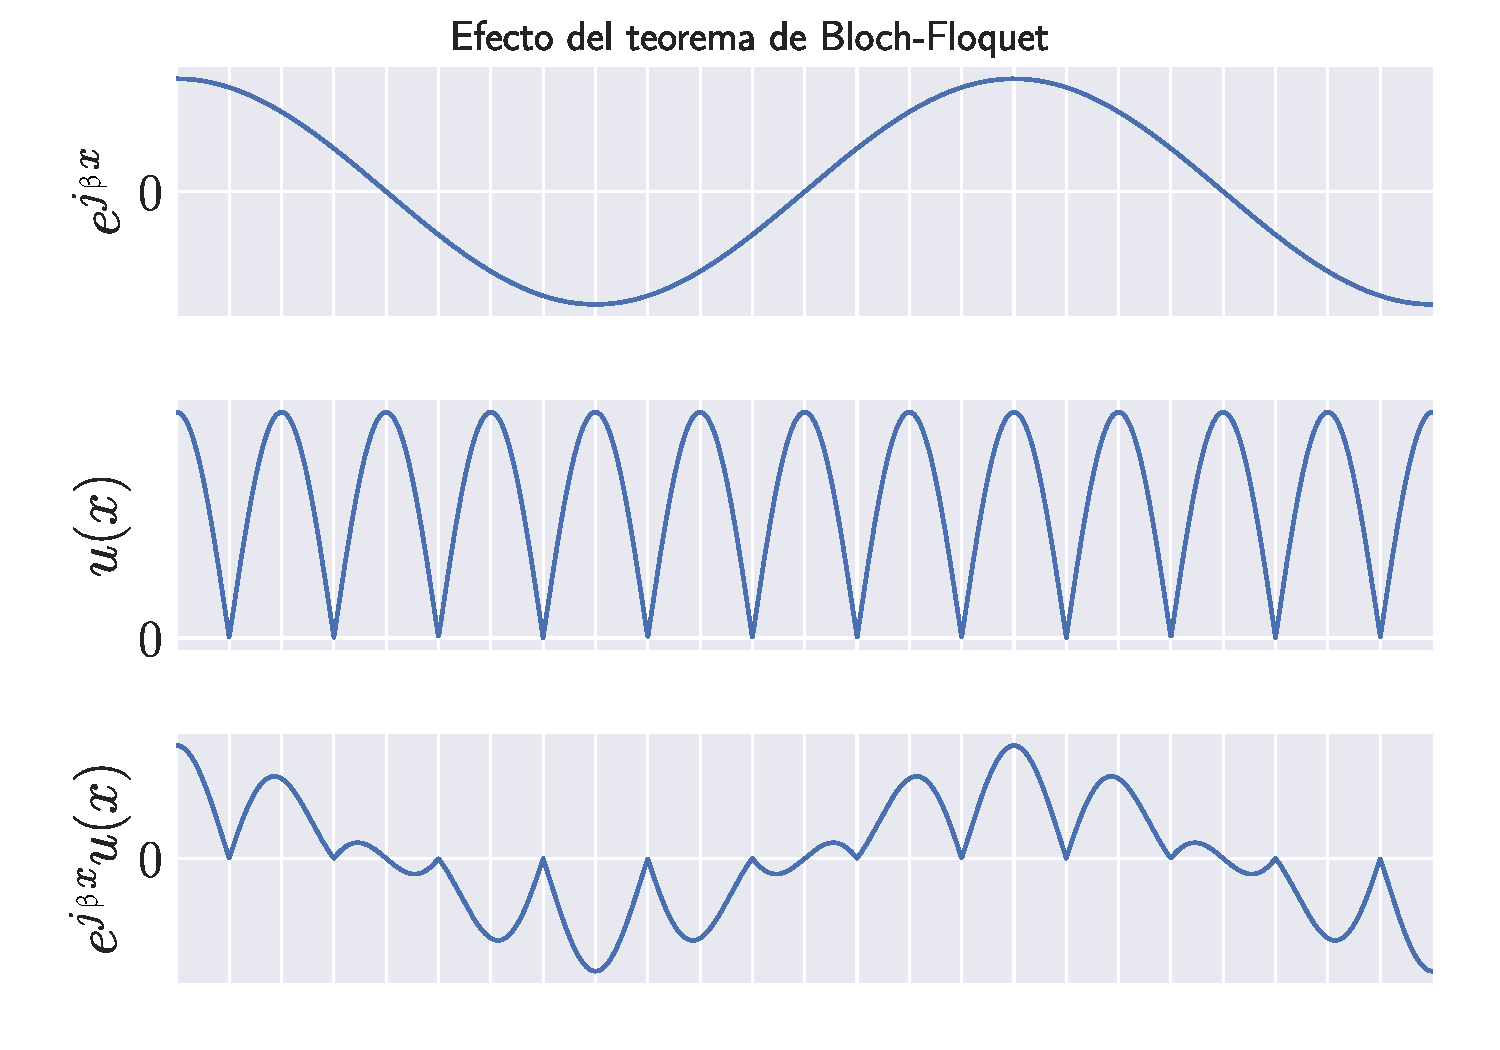
\includegraphics[width=0.8\textwidth]{Fundamentos/bloch.pdf}
	\caption{Comportamiento de una onda monocromática sobre un medio periódico. La función $u(\vec{r})$ tiene un comportamiento de igual periodicidad que el medio.}
	\label{fig:bloch-periodico-1d}
\end{figure}

La idea intuitiva detrás del resultado radica en que si la estructura es infinitamente periódica, con celdas unitarias idénticas, las mismas deberían ser indistinguibles, por lo que los campos electromagnéticos presentarían también un comportamiento periódico, a excepción de un corrimiento de fase. Por lo tanto, se puede escribir:

\begin{equation}
	\label{eq:comportamiento-periodico-campo-bloch}
	E(x,y,z+d) = e^{j \beta d} E(x,y,z)
\end{equation}

donde $\beta$ es la constante de propagación en el medio periódico, considerando que no hay pérdidas ($\gamma = \beta$) \cite{Capolino:TheoryPhenomenaMetamaterials}. El valor de la diferencia entre los campos en dos bordes de una celda unitaria, entonces, es $\beta d$, que puede reducirse al rango $[-\pi,\pi]$, de modo que los posibles valores de $\beta$ son $[-\pi/d,\pi/d]$, que son los límites de la celda de Brillouin descripta antes. La generalización para el comportamiento en dos dimensiones está íntimamente ligado a la definición de la zona de Brillouin del material analizado.

Si una onda plana incide sobre un medio periódico dispuesto en la dirección ortogonal al vector de propagación, el efecto es intuitivo, como se puede ver en la figura \ref{fig:bloch-ortogonal}. En este caso, la periodicidad se da sobre el eje $z$, y la constante de propagación en esa coordenada es nula, por lo que no hay diferencia de fase entre los elementos dispuestos periódicamente (la diferencia de fase se da, para la onda incidente dibujada, en la dirección $y$).

\begin{figure}[htp]
	\centering
	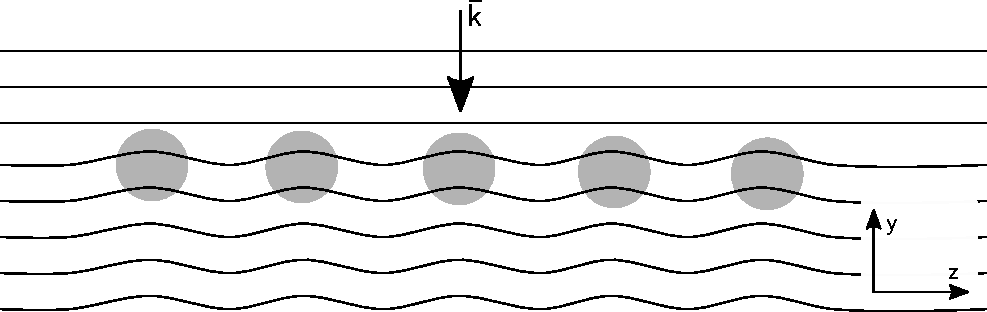
\includegraphics[width=0.8\textwidth]{Fundamentos/bloch-ortogonal.pdf}
	\caption{Comportamiento de una onda monocromática que incide en forma perpendicular a un medio periódico unidimensional.}
	\label{fig:bloch-ortogonal}
\end{figure}


\section{Relación y diagrama de dispersión}
\label{sec:diag-de-dispersion}
%%%%
% Libro de rahmat. Pagina 46.
% Zona de brillouin. Rahmat, libro, pagina 31.
% Diagrama de dispersión. Página 67 Rahmat. Caloz: pagina 106.
% Impedancia de Bloch: Caloz, pagina 113
% Tesis Choi, pag 82.
% Tesis Kovacs, pag 13.
% Venkateswaran, pag 26.
% Tesis Zheng, pag 5-8

Las estructuras periódicas se usan comúnmente en microondas, principalmente como filtros, dado que pueden ser modeladas como líneas de transmisión cargadas, lo que permite describir las características que comparten con los mismos, utilizando nomenclaturas similares para fenómenos similares.

Una línea de transmisión infinita cargada periódicamente puede analizarse planteando las matrices ABCD\footnote{Las matrices ABCD son matrices que relacionan la corriente y la tensión a la entrada con la corriente y la tensión a la salida de un sistema. De esta manera, los parámetros A y D son adimensionales, el parámetro B tiene dimensiones de impedancia, y el parámetro C tiene dimensiones de admitancia.} de cada celda unitaria, considerando puntual el efecto de carga que impone la geometría, de forma que:

\begin{equation}
	\begin{bmatrix}
		V_n \\
		I_n
	\end{bmatrix}
	=
	\begin{bmatrix}
		A & B \\
		C & D
	\end{bmatrix}
	\begin{bmatrix}
		V_{n+1} \\
		I_{n+1}
	\end{bmatrix}
\end{equation}

Si se considera que la línea está cargada con una impedancia y una admitancia, como indica la figura \ref{fig:linea-transm-cargada-periodica}, entonces se puede dividir a cada celda unitaria en secciones diferenciadas, y multiplicar las matrices $\text{ABCD}_{i}$ de cada sección para obtener la matriz ABCD que corresponde a la celda unitaria completa.

\begin{figure}[htp]
	\centering
	\begin{circuitikz} \draw
		(0,0) -- (1,0)node[midway,scale=2,fill=white]{$\cdots$}
			to [transmission line,-o,v=$d/2$] (5,0)
			-- (7,0)
		(0,2) -- (1,2)node[midway,scale=2,fill=white]{$\cdots$} 
			to [transmission line,-o,l_=$Z_0$] (5,2)
			to [generic,l=$Z$] (7,2)
			to [generic,l=$Y$] (7,0)
			-- (7.5,0)
			to [transmission line,o-,v=$d/2$]
			(10,0) -- (11,0)node[midway,scale=2,fill=white]{$\cdots$}
		(7,2) -- (7.5,2)
			to [transmission line,-o,l_=$Z_0$]
			(10,2) -- (11,2)node[midway,scale=2,fill=white]{$\cdots$};
%			to [C,l=$C'_R \Delta_z$] (7,0)
%		-- (9,0) to [L,l_=$L'_L / \Delta_z$] (9,2)
%		-- (7,2)
%		(9,2) -- (11,2)
%		to [R,l=$R / \Delta_z$] (11,0)
%		-- (9,0)
%		(11,0) -- (12,0) -- (13,0)node[midway,scale=2,fill=white]{$\cdots$}
%		(11,2) -- (12,2) -- (13,2)node[midway,scale=2,fill=white]{$\cdots$};
	\end{circuitikz}  	
	\caption{Circuito equivalente de porción de línea de transmisión cargada, de longitud $d$.}
	\label{fig:linea-transm-cargada-periodica}
\end{figure}

\begin{enumerate}
	\item La primera mitad de la línea de transmisión, de largo $d/2$, cuya matriz ABCD es, considerando $Z_0$ su impedancia característica y $\beta_{TL}$ la constante de propagación \cite{Pozar:MwEngineering}:
	\begin{equation}
		\begin{bmatrix}
			A & B \\
			C & D
		\end{bmatrix}_{1,3}
		=
		\begin{bmatrix}
			\cos(\beta_{TL} d/2) & j Z_0 \sin(\beta_{TL} d/2) \\
			j Y_0 \sin(\beta_{TL} d/2) & \cos(\beta_{TL} d/2)
		\end{bmatrix}
	\end{equation}
	\item La carga, que comprende a la impedancia $Z$ y la admitancia $Y$ asociada a la línea de transmisión. La matriz resulta:
	\begin{equation}
		\begin{bmatrix}
			A & B \\
			C & D
		\end{bmatrix}_{2}
		=
		\begin{bmatrix}
			1+ZY & Z \\
			Y & 1
		\end{bmatrix}
	\end{equation}
	\item La segunda mitad de la línea de transmisión, de largo $d/2$, de igual expresión que la primera mitad.
\end{enumerate}

Si se considera que la relación entre las tensiones y corrientes de entrada y salida, respectivamente, están relacionadas por el factor de propagación $e^{-\gamma d}$, donde $\gamma$ es el módulo del vector de onda en el medio metamaterial que se quiere obtener, entonces:

\begin{equation}
	\begin{bmatrix}
		V_n \\ I_n
	\end{bmatrix}
	=
	\begin{bmatrix}
	A & B \\
	C & D
	\end{bmatrix}
	\begin{bmatrix}
	V_{n+1} \\
	I_{n+1}
	\end{bmatrix}
	=
	\begin{bmatrix}
	V_{n+1}e^{\gamma d} \\ 
	I_{n+1}e^{\gamma d}
	\end{bmatrix}
	\implies
	\begin{bmatrix}
	A-e^{\gamma d} & B \\
	C & D-e^{\gamma d}
	\end{bmatrix}
	\begin{bmatrix}
	V_{n+1} \\ I_{n+1}
	\end{bmatrix}
	= 0
\end{equation}

La existencia de una solución no trivial del sistema de ecuaciones planteado requiere que el determinante de la matriz se anule. Recordando, además, que en las redes recíprocas, $AD-BC=1$ \cite{Pozar:MwEngineering}:

\begin{subequations}
	\begin{align}
		AD + e^{2 \gamma d} - (A+D)e^{\gamma d}-BC = 0 \implies &1+e^{2\gamma d}-(A+D)e^{\gamma d} = 0 \\
		&\cosh (\gamma d) = \frac{A+D}{2}
	\end{align}
\end{subequations}

Reemplazando los valores de A y D de la matriz de transmisión de la celda unitaria completa, que surge de la multiplicación de las matrices de transmisión que la componen:

\begin{equation}
\cosh (\gamma d) = \frac{Y Z}{2} \cos{\left (\beta_{TL} d \right )} + \frac{i Y Z_{0}}{2} \sin{\left (\beta_{TL} d \right )} + \frac{i Z}{2 Z_{0}} \sin{\left (\beta_{TL} d \right )} + \cos{\left (\beta_{TL} d \right )}
\end{equation}

Dado que $\gamma = \beta -j\alpha$ es la constante de onda en el material, resulta conveniente considerar el caso en que no hay comportamientos exponenciales negativos para las ondas que los atraviesan, de modo que $\alpha=0$ \footnote{$\cosh (\gamma d) = \cosh(\beta d)\cos(\alpha d) + j \sinh(\beta d) \sin(-\alpha d) = \cosh (\beta d)$}. Se obtiene, entonces, la ecuación de dispersión para una dimensión:

\begin{align}
	\label{eq:relacion-de-dispersion-general}
	cosh(\beta d) = \frac{Y Z}{2} \cos{\left (\beta_{TL} d \right )} + \frac{i Y Z_{0}}{2} \sin{\left (\beta_{TL} d \right )} + \frac{i Z}{2 Z_{0}} \sin{\left (\beta_{TL} d \right )} + \cos{\left (\beta_{TL} d \right )}
\end{align}

El diagrama de dispersión es un gráfico que muestra la relación entre la frecuencia angular, $\omega$, y el módulo del vector de onda, $|\vec{\beta}|$. En la ecuación \ref{eq:relacion-de-dispersion-general}, si se reemplaza $\beta_{TL}$ por $\omega/v_p$, con $v_p$ la velocidad de fase de una onda monocromática que viaja por la línea de transmisión, se obtiene la relación buscada. Para el caso en que no existen discontinuidades periódicas, sino que la onda se desplaza sobre un medio homogéneo sin pérdidas, la relación es independiente de la frecuencia: $v_p = c/\sqrt{\epsilon_r \mu_r}$, la velocidad de la luz en el medio.

Para el caso bidimensional, el análisis es similar, aunque se obtiene mayor información si se analizan simultáneamente las componentes ortogonales del vector $\vec{\beta}$. Para el caso de un medio homogéneo, el diagrama de dispersión es un cono, denominado comúnmente ``cono de luz", como se muestra en la figura \ref{fig:diagrama-dispersion-vacio-3d}, que surge de la expresión $\omega = c \sqrt{\beta_x^2 + \beta_y^2}$.

\begin{figure}[htp]
	\centering
	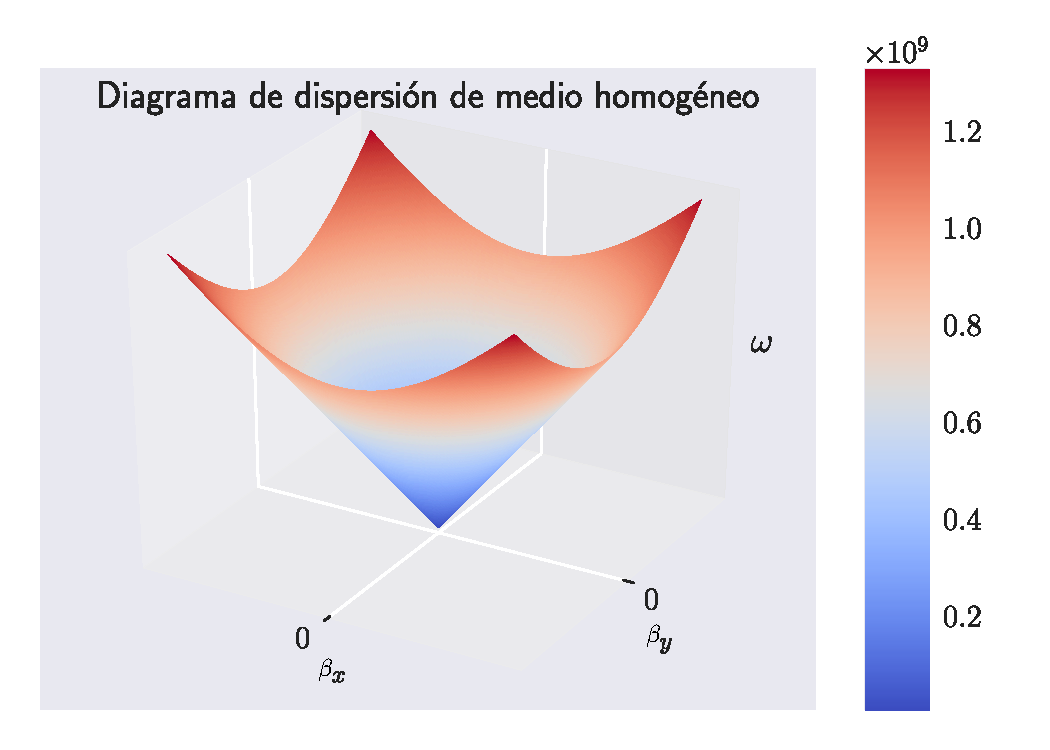
\includegraphics[width=0.7\textwidth]{Fundamentos/plot-cono-luz.pdf}
	\caption{Gráfica del diagrama de dispersión tridimensional para el caso del vacío, denominado cono de luz.}
	\label{fig:diagrama-dispersion-vacio-3d}
\end{figure}

El análisis tridimensional del diagrama de dispersión de una estructura periódica bidimensional posee, en muchos casos, información redundante, y su lectura puede ser complicada.

En función de lo explicado en la sección \ref{sec:celdas-unitarias}, y en base a lo analizado sobre el teorema de Bloch, resulta evidente que un análisis del comportamiento de una onda plana que viaja por un material periódico se reduce a comprender el mismo en una región limitada del espacio, conocida como la zona de Brillouin. Si, además, existen simetrías, las mismas permiten reducir aún más el espacio de análisis, dando lugar a la zona irreducible de Brillouin, de la cual las demás regiones del material son reflexiones y traslaciones. Sobre esta zona se presentan todos los posibles vectores de onda del espacio.

\begin{figure}[h]
	\centering
	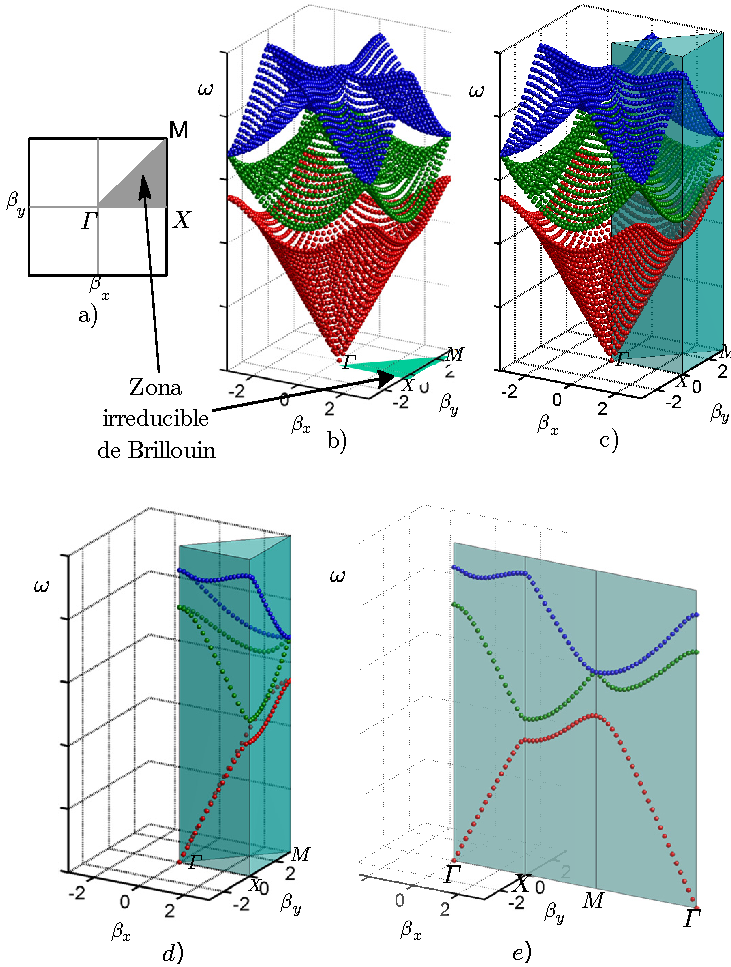
\includegraphics[width=0.9\textwidth]{Fundamentos/diagrama-dispersion-deduccion.pdf}
	\caption{Gráficas ilustrativas del análisis del diagrama de dispersión sobre la zona de Brillouin [Raymond C. Rumpf, diapositivas del curso \textit{21st Century Electromagnetics}].}
	\label{fig:diagrama-dispersion-completo-deduccion}
\end{figure}

Para una superficie bidimensional, el análisis requiere que para cada punto dentro de la zona de Brillouin, se analice el valor de $\omega$ correspondiente. Para un caso sencillo como el mostrado en la figura \ref{fig:rectangulo-cuadrado}, el cálculo se debe realizar para todas las combinaciones posibles de valores de $\beta_x$ en el intervalo $[0,\pi/d_x]$ y de $\beta_y$ en el intervalo $[0,\pi/d_y]$. Este análisis da lugar a el diagrama de dispersión o diagrama de bandas completo, que sigue requiriendo una representación tridimensional, como se muestra en las figura \ref{fig:diagrama-dispersion-completo-deduccion}c), que explicita que el análisis del diagrama completo sobre una celda unitaria se puede realizar sobre la zona irreducible de Brillouin. Una simplificación muy utilizada, que reduce la cantidad de información a considerar, aunque vuelve incompleto el diagrama, es la mostrada en la figura d), donde se analizan únicamente los valores del diagrama de dispersión sobre los bordes de la zona irreducible de Brillouin. De esta forma, resulta fácil expresar un diagrama de dispersión en un gráfico bidimensional, como se muestra en la figura e). Los puntos denominados $\Gamma$, X y M representan los vértices de la zona de análisis.

Para el caso particular del vacío, el diagrama de dispersión simplificado, calculado a partir del que se observa en la figura \ref{fig:diagrama-dispersion-vacio-3d}, es el mostrado en la figura \ref{fig:diagrama-dispersion-vacio-2d}.

\begin{figure}[h]
	\centering
	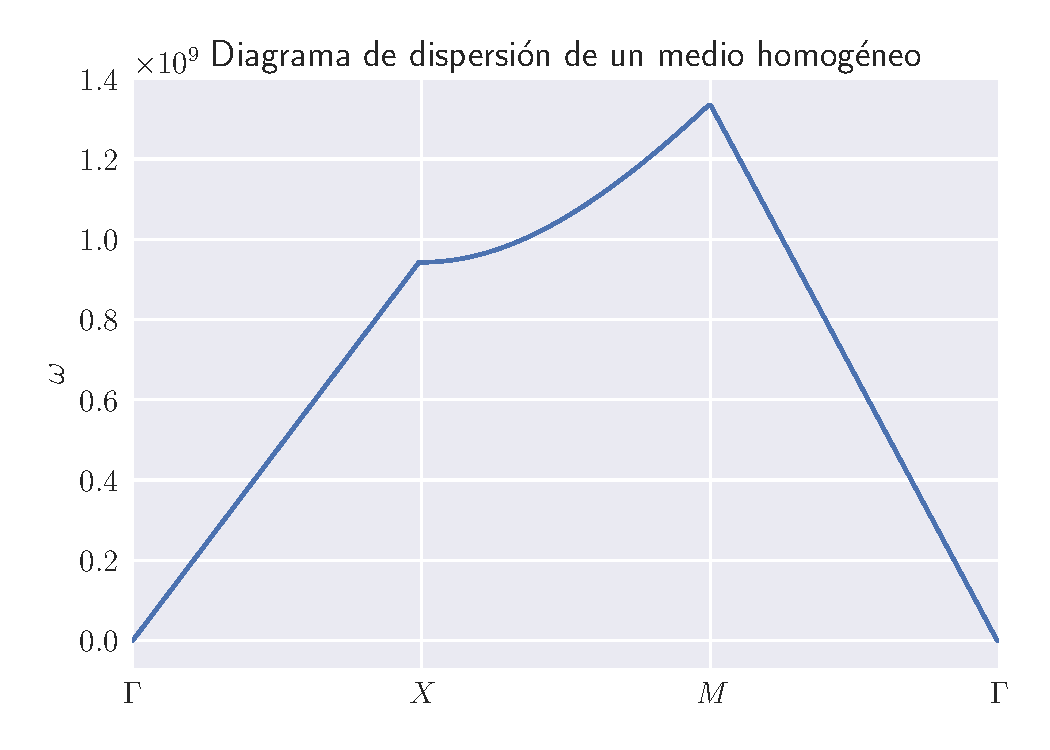
\includegraphics[width=0.6\textwidth]{Fundamentos/diag-dispersion-vacio-2d.pdf}
	\caption{Diagrama de dispersión del vacío, calculado a partir de su representación tridimensional mostrada en la figura \ref{fig:diagrama-dispersion-vacio-3d}. Para el vacío no existen modos de propagación.}
	\label{fig:diagrama-dispersion-vacio-2d}
\end{figure}

Una explicación intuitiva sobre el comportamiento en cada punto de la frontera de la zona irreducible de Brillouin se puede observar en la figura \ref{fig:explicacion-zona-brillouin}. En el centro de la misma se ubica una celda de Brillouin, que equivale a una celda de Wigner-Seitz del espacio recíproco. En la misma se destaca la zona irreducible de Brillouin de una celda cuadrada, cuyos vértices se denominan $\Gamma$, $X$ y $M$. Alrededor de la gráfica de la zona de Brillouin, se muestra una representación gráfica de una onda plana incidente, para el modo más bajo (la frecuencia más baja de las posibles).

La gráfica de la zona de dispersión comienza en el punto $\Gamma$ de la zona irreducible de Brillouin, que corresponde a un valor de $\beta_x = 0$ y $\beta_y = 0$, por lo que no hay variación espacial del valor de los campos. El recorrido de las abscisas continúa hacia el punto $X$, que corresponde a un valor de $\beta_x$ equivalente a $\pi / d$, con $d$ la periocidad en $x$, como se muestra en la figura. Los valores intermedios entre $\Gamma$ y $X$ representan valores de $\beta_x$ cada vez mayores, mientras se mantiene la frecuencia espacial en el eje $y$ en cero. El aumento de la frecuencia espacial da lugar a longitudes de onda menores.

Una vez alcanzado el punto $X$ de la zona irreducible de Brillouin, el recorrido continúa hacia el punto $M$, donde el cambio se da sólo para el valor de $\beta_y$, con $\beta_x$ fijo en $\pi / a$. Esto indica una incidencia oblicua, como se esquematiza en las figuras que rodean a la zona de Brillouin.

El recorrido se completa con el camino entre el punto $M$ y el punto $\Gamma$, donde ahora los valores de $\beta_x$ y $\beta_y$ disminuyen simultáneamente, a la misma velocidad, y en la dirección correspondiente a $45^\circ$, como se observa en las gráficas de la zona superior izquierda de la figura.

\begin{figure}[h]
	\centering
	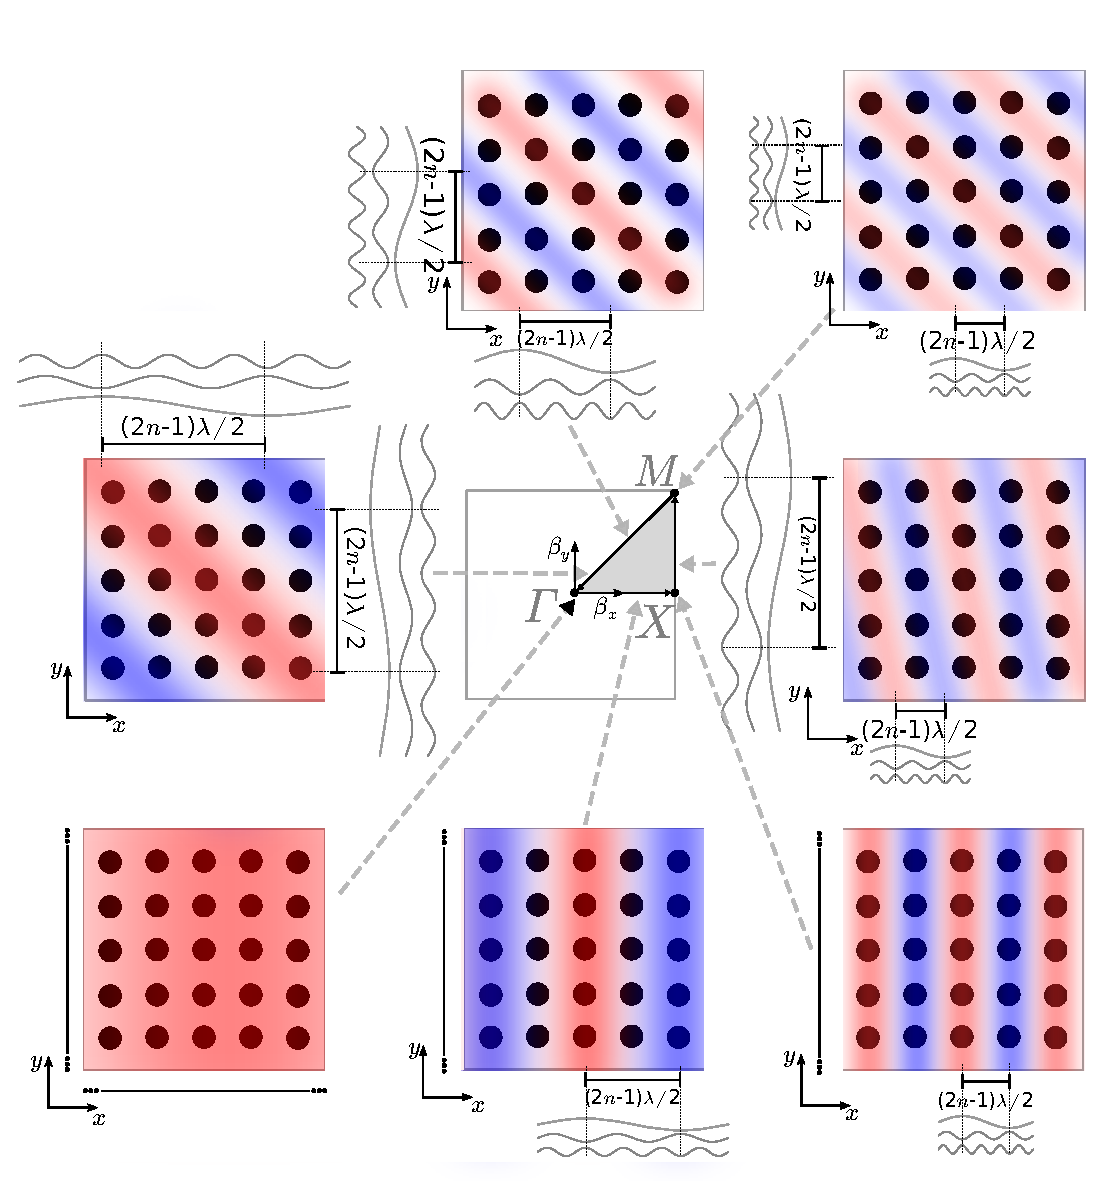
\includegraphics[width=0.9\textwidth]{Fundamentos/Fisica-DiagramaDeFase.pdf}
	\caption{Explicación gráfica de la incidencia de ondas planas para cada punto del borde de la zona irreducible de Brillouin que da lugar al diagrama de dispersiñon.}
	\label{fig:explicacion-zona-brillouin}
\end{figure}

Se debe tener en cuenta que, dado que existen distintos modos, frecuencias de incidencia mayores darían lugar a modos superiores, que compartirían el valor de $\beta_i$ con los modos inferiores. Esto se debe a que la diferencia de fase medida en los extremos de la celda unitaria de la red de Bravais no tiene en cuenta la cantidad de ciclos que le dieron origen (es decir, una diferencia de fase de $\phi$ da lugar al mismo $\beta_i$, $i=x,y$ que una diferencia de $\pi+2 n \pi$). Esto es esquematizado en la parte superior y los lados de las figuras que representan al arreglo periódico.

